\chapter{相关工作}
本章内容概括人机重定向相关研究内容，并介绍现有人机重定向算法原理，主要分为基于优化的方法、基于学习的方法以及优化与学习结合的混合方法
这三类进行介绍。同时介绍Transformer架构和其在人体骨骼点序列里面的应用。
% \section{基于优化的方法}
% 论文主体是毕业论文的主要部分，必须言之成理，论据可靠 \cite{tighe2013finding}，严格遵循本学科国际通行的学术规范。在写作上要注意结构合理、层次分明、重点突出。

% 本章举例说明本模板中图片，表格及公式的插入及引用方法 \cite{liu2011sift}。

% \subsection{图片格式举例}

% 图片的分辨率至少300个像素，建议格式为.png。图 \ref{fig1} 显示……，图 \ref{subfig1} 表明……。

% \subsubsection{单张图片}
% \begin{figure}[h]
% 	\centering
% 	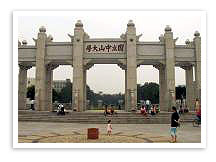
\includegraphics[width=0.8\textwidth]{figure/fig1.png}
% 	\caption{标题} 
% 	\label{fig1}
% \end{figure}

% \subsubsection{多张子图}
% \begin{figure}[h!] % image examples & compare
% 	\begin{subfigure}{0.55\textwidth}
% 		\centering
% 		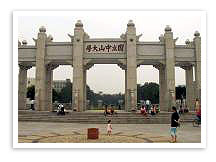
\includegraphics[width=0.5\textwidth]{figure/fig1.png}
% 		\caption{子图1}
% 		\label{subfig1}
% 	\end{subfigure}
% 	\begin{subfigure}{0.55\textwidth}
% 		\centering
% 		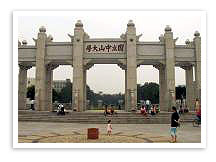
\includegraphics[width=0.5\textwidth]{figure/fig1.png} 
% 		\caption{子图2}
% 		\label{subfig2}
% 	\end{subfigure}
% 	\begin{subfigure}{0.55\textwidth}
% 		\centering
% 		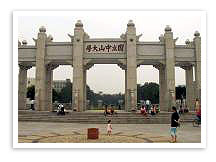
\includegraphics[width=0.5\textwidth]{figure/fig1.png}
% 		\caption{子图3}
% 		\label{subfig3}
% 	\end{subfigure}
% 	\begin{subfigure}{0.55\textwidth}
% 		\centering
% 		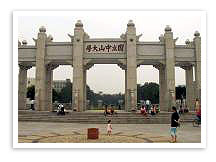
\includegraphics[width=0.5\textwidth]{figure/fig1.png} 
% 		\caption{子图4}
% 		\label{subfig4}
% 	\end{subfigure}
% 	\caption{多子图}
% 	\label{subfig}
% \end{figure}




% \subsection{表格举例}
% 表 \ref{tab1} 表示……。
% \begin{table}[h]
% 	\centering
% 	\caption{国际单位制中具有专门名称的导出单位}		
% 	\label{tab1}
% 	\begin{tabular}{c|c|c|c}
% 		\toprule[2pt]
% 		量的名称 & 单位名称 & 单位符号 & 其他表示式例\\
% 		\midrule[2pt]
% 		频率	& 赫［兹］	& Hz	&$s^{-1}$ \\
% 		\hline                                        %细横线
% 		力；重力 	& 牛［顿］	& $N$	 & $kg·m/s^2$ \\
% 		\hline                                         %细横线
% 		压力，压强；应力	& 帕［斯卡］	&$Pa$	&$N/m^2$ \\
% 		\bottomrule[2pt]
% 	\end{tabular}
% \end{table}

% \subsection{公式举例}
% \label{sec:formula}
% 没有编号的公式:
% \begin{equation*}
% \bm{z}^{(l)} = \bm{W}^{(l)}\bm{a}^{(l-1)} + \bm{b}^{(l)} 
% \end{equation*}

% 公式中含有中文:
% \begin{equation}
% \mbox{像素准确率} = \sum_{i=1}^{n_{cl}}n_{ii} / \sum_{i=1}^{n_{cl}}t_i
% \end{equation}

% 公式中含有矩阵:
% \begin{equation}
% \label{eq1}
% \textbf{H} = \begin{bmatrix}
% I*\bm{x}_i \\ \textbf{h}
% \end{bmatrix}
% \end{equation}

% 多行公式：
% \begin{align} 
% \hat{\bm{R}}_r 
% & =   \frac{1}{N_s} \sum_{i=1}^{Ns} \bm{r}_i \bm{r}_i^T  \label{Eq-2-a} \\
% & =   \frac{1}{N_s} \sum_{i=1}^{Ns} \bm{r}_i \bm{r}_i^T  \nonumber \\
% & =   \frac{1}{N_s} \sum_{i=1}^{Ns} \bm{r}_i \bm{r}_i^T  \label{Eq-2-c},
% \end{align}

% 引用：公式 \eqref{eq1} ……，\eqref{Eq-2-a}……。

% 更多的数学公式编辑方法，请参考根文件下“LaTex学习文档”中的文献1和文献3。

% \subsection{算法举例}


% \begin{algorithm}[h]
% 	\KwIn{$m$个训练样本}
% 	\lFor{$l=1$ \emph{\KwTo} $n_l$}{
% 		初始化：$\Delta \bm{W}^{(l)}=0$，$\Delta \bm{b}^{(l)}=0$}
% 	\ForEach{训练样本}{
% 		\lFor{$l=1$ \emph{\KwTo} $n_l-1$}{
% 			前向传播：$\bm{z}^{(l+1)}=\bm{W}^la^l+\bm{b}^l$,$\bm{a}^{(l+1)}=f(\bm{z}^{(l+1)})$}
% 		输出误差计算：$\delta^{(n_l)} = \frac{\partial}{\partial \bm{z}^{(n_l)}} J(\bm{W},\bm{b};\bm{x},y)$\;
% 		\lFor{$l=n_l-1$ \emph{\KwTo} $1$}{
% 			后向传播：$\delta^{(l)} = \bigl((\bm{W}^{(l)})^T \delta^{(l+1)}\bigr)f'(\bm{z}^{(l)})$}
% 		\ForAll{层l}{
% 			计算梯度：$\nabla_{\bm{W}^{(l)}}J(\bm{W},\bm{b};\bm{x},y)=\delta^{(l+1)}(\bm{a}^{(l)})^T$ \\
% 			\hspace{60pt}$\nabla_{\bm{b}^{(l)}}J(\bm{W},\bm{b};\bm{x},y)=\delta^{(l+1)}$\;
% 			累加梯度：$\Delta \bm{W}^{(l)} \leftarrow \Delta \bm{W}^{(l)} + \nabla_{\bm{W}^{(l)}}J(\bm{W},\bm{b};\bm{x},y)$; \\
% 			\hspace{60pt}$\Delta \bm{b}^{(l)} \leftarrow \Delta \bm{b}^{(l)} + \nabla_{\bm{b}^{(l)}}J(\bm{W},\bm{b};\bm{x},y)$\;
% 		}
% 	}
% 	\ForAll{层$l$}{
% 		更新权重：$\bm{W}^{(l)} \leftarrow \bm{W}^{(l)} - \alpha \biggl[\frac 1m \Delta \bm{W}^{(l)}]$ \\
% 		\hspace{60pt} $\bm{b}^{(l)} \leftarrow \bm{b}^{(l)} - \alpha \biggl[\frac 1m \Delta \bm{b}^{(l)}\biggr]$
% 	}
% 	\caption{梯度下降算法}
% 	\label{sgd}
% \end{algorithm}

% 算法 \ref{sgd}……。

% \subsection{例子}
% \begin{eg}
% 	这是一个例子。
% 	\label{eg1}
% \end{eg}
% 例 \ref{eg1} ……。

% \subsection{证明}
% \begin{proof}
% 证明过程
% \end{proof}

% \subsection{定理}
% \begin{theorem}
% 	这是一个定理。
% 	\label{th1}
% \end{theorem}
% 定理 \ref{th1} ……。

% \subsection{命题}
% \begin{proposition}
% 	这是一个命题。
% 	\label{pro1}
% \end{proposition}
% 命题 \ref{pro1} ……。

% \subsection{引理}
% \begin{lemma}
% 	这是一个引理。
% 	\label{lem1}
% \end{lemma}
% 引理 \ref{lem1} ……。

% \subsection{推论}
% \begin{corollary}
% 	这是一个推论。
% 	\label{cor1}
% \end{corollary}
% 推论 \ref{cor1} ……。

% \subsection{定义}
% \begin{definition}
% 	这是一个定义。
% 	\label{def1}
% \end{definition}
% 定义 \ref{def1} ……。

% \subsection{标记}
% \begin{remark}
% 	这是一个标记。
% 	\label{rem1}
% \end{remark}
% 标记 \ref{rem1} ……。



\section{基于优化的方法}
\subsection{基本原理}
基于优化的算法将人机运动重定向视为一个在特定约束条件下的数学寻优问题。
其核心逻辑是构建一个目标函数，通过数学求解器（Solver）在每一帧数据中计算出一组机器人关节角度，
使得机器人的末端执行器（End Effector）与人类手部对应关键点之间的欧式距离最小化。
该类方法通常基于逆运动学（Inverse Kinematics, IK）理论。
给定人类手部的关键点坐标序列 $H = \{h_1, h_2, \dots, h_n\}$，目标是求解机器人关节角度矢量 $\theta$，
使得机器人的末端执行器位置 $f(\theta)$ 与对应的人类关键点 $h$ 之间的距离函数 $D$ 最小化。
其标准的数学表达形式如下：$$\min_{\theta} \|f(\theta) - \phi(h)\|^2 + \lambda R(\theta)$$其中，$\phi$ 为空间映射函数，$R(\theta)$ 为正则化项（如关节速度平滑约束或偏离标准姿态的惩罚项），
$\lambda$ 为平衡系数。求解过程通常涉及雅可比矩阵（Jacobian Matrix）的迭代计算。
\subsection{基于重投影的实时优化 (AnyTeleop)}
AnyTeleop 是一种典型的基于视觉观测和实时优化的重定向框架。它通过构建统一的运动学流形，
将不同结构的灵巧手映射到同一参数空间中。该方法利用高性能求解器在极短的时间内完成逆向寻优，
其最大的特点是无需离线预训练，即可实现从单目相机输入到异构灵巧手动作的实时转换，展现了极佳的即插即用特性。
\subsection{基于能量函数的全身映射}
另一类著名方法侧重于全局一致性，通过设计复杂的能量函数（Energy Function）来描述人机之间的位姿相似度。
这类方法不仅考虑末端位置的对齐，还引入了关节限位、自碰撞规避以及重心平衡等物理约束。例如，在早期的类人机器人重定向研究中，
研究者通过拉格朗日乘子法处理等式与不等式约束，确保了机器人在追踪人类动作时的物理稳定性。
\subsection{优缺点}
优点：
平台无关性：算法逻辑基于通用的运动学描述，能够快速适配不同自由度（DoF）配置的机器人平台。
无需训练数据：不需要大规模的手动标注数据集，极大降低了系统的前期开发成本。
物理准确性：通过显式添加硬约束（Hard Constraints），可以严格保证生成的动作不超出机器人的机械极限。

缺点：
局部最优陷阱：受限于非线性优化的本质，求解器容易收敛至局部极小值，导致生成的动作出现不连续的跳变。
计算开销与精度的矛盾：为了提高实时性，往往需要限制迭代次数，这会直接导致末端映射的精度下降。
时序平滑度缺失：由于该类方法多针对单帧进行独立优化，忽略了动作的内在惯性，输出序列往往存在高频抖动
\section{基于学习的方法}
\subsection{基本原理}
基于学习的方法利用深度神经网络强大的非线性拟合能力，
试图直接建立从人类手部姿态特征空间到机器人关节角度空间（或控制参数空间）的映射函数。

该类方法的核心思想是将重定向任务建模为回归问题。通过构建深度神经网络（如多层感知机 MLP 或卷积神经网络 CNN），
在海量的人机动作配对数据集上进行监督学习或自监督学习。
其基本数学形式可以表示为：$$\theta = \mathcal{N}(H; \omega)$$其中，$H$ 为输入的人手关键点特征向量，
$\omega$ 为待优化的网络参数。在训练过程中，通过定义相似度损失函数（Similarity Loss）和物理约束损失，
引导网络自动提取人手运动中的高维语义信息，并将其转化为目标机器人的运动指令。
\subsection{基于重定向网络的手部映射}
DexPilot 是一种代表性的数据驱动重定向框架。它利用深度学习模型从单目视觉输入中提取人手姿态，
并采用点云匹配或关键点回归的方式，将复杂的指尖运动映射到高自由度的灵巧手上。
该方法的突出特点是利用大规模的合成数据集进行预训练，
使得系统在处理光照变化和遮挡时表现出极强的鲁棒性，能够实现高精度的实时灵巧操作。
\subsection{跨域语义对齐映射 (TeachNet)}
TeachNet 引入了端到端（End-to-End）的学习思路，通过设计一种视觉识别与重定向协同优化的架构，
解决了人手与机器人手形状异构带来的特征失配问题。该方法通过构建共享的特征嵌入空间，
强制模型学习人手关键点与机器人指尖之间的几何对应关系。
TeachNet 证明了在大规模数据驱动下，模型可以绕过复杂的解析解算，直接输出符合人类意图的平滑抓取动作。
\subsection{优缺点}
优点：
推理速度极快：模型训练完成后，前向传播的计算开销极低，能够轻松满足数百赫兹（Hz）的实时控制需求。
鲁棒性强：在面对视觉输入噪声、关键点缺失或部分遮挡时，深度模型通常具有比几何优化更好的容错能力。
精度上限高：通过增加模型参数量和训练数据多样性，可以捕捉到优化方法难以建模的复杂动作细节。

缺点：
泛化性能受限：模型通常高度依赖于特定的机器人硬件配置，当迁移到不同结构的灵巧手时，往往需要重新采集数据并训练。
数据依赖严重：高质量、大规模的人机动作配对数据获取成本极高，且模型容易受到训练数据分布偏差的影响。
不可解释性：黑盒化的神经网络难以保证生成的动作始终符合严格的物理约束，偶尔会出现违反关节限位或产生物理碰撞的非预测行为。
\section{结合了优化与学习的方法}
为了克服纯优化方法易陷入局部最优以及纯学习方法泛化性较差的局限，
研究者开始探索将深度学习的感知能力与数值优化的约束处理能力相结合的混合框架。
\subsection{基本原理}
该类方法的核心思想是利用神经网络为优化过程提供高质量的先验知识。通常通过编码器将人类动作映射到低维的隐空间（Latent Space），
并在该空间内利用神经网络的输出作为初始值，辅助数值求解器进行迭代优化。
其数学本质是利用学习到的运动规律来缩小优化的搜索范围，使求解过程既能快速收敛，
又能有效跳出局部极小值的陷阱，从而兼顾了推理效率与平台泛化性。
\subsection{基于图神经网络加速的初始值预测}
由于人手与机器人手的拓扑结构具有天然的图属性，部分研究采用图神经网络（GNN）及其变体来提取关节间的空间层级特征。
通过改进图卷积算子或引入更灵活的动态图结构，模型能够学习不同自由度之间的协同映射关系，
并为优化算法提供极具物理意义的初始关节向量。
这种基于图结构的初始值辅助机制显著减少了逆运动学求解所需的迭代次数，在保持高精度的同时提升了系统的实时响应频率。
\subsection{C3PO}
C3PO 是一种典型的三阶段循环优化架构。它首先利用深度网络在隐空间内预测目标姿态的特征表示，
随后通过循环一致性约束和几何优化层对结果进行精修。
C3PO 的核心贡献在于它将高维的运动空间映射问题转化为隐空间内的特征对齐问题，
既保留了学习方法对视觉噪声的容错性，又通过优化闭环确保了生成的动作符合机器人底层的物理拓扑约束。
\subsection{优缺点}
优点：
协同优势明显：解决了纯优化方法对“冷启动”初始值的依赖，同时弥补了纯学习方法在推理时间和跨平台部署上的短板。
鲁棒性与精度兼备：神经网络提供的全局先验与优化层提供的局部约束相结合，使系统在复杂交互任务中表现更稳健。
主流技术趋势：在处理异构灵巧手映射时，展现出了比单一路径更强的适配能力。

缺点：
计算时延叠加：尽管优化迭代次数减少，但模型前向传播与求解器运行的总耗时仍不可忽视。
时序平滑度缺失：现有的混合方法大多仍采用逐帧（Frame-by-frame）处理逻辑，未能充分利用连续输入帧之间的时空相关信息。 由于忽略了帧间依赖关系，在面对视觉抖动或高速运动时，生成的机器人动作序列仍存在连续性不足、不够平滑的问题。
\section{Transformer架构简述}
Transformer 架构自提出以来，因其卓越的序列建模能力，已成为处理时序数据（如语音、文本及机器人动作序列）的核心技术方案。
其核心优势在于摒弃了传统循环神经网络的顺序计算模式，转而采用全局并行的注意力机制。
\subsection{Transformer的提出}
Transformer 最初由 Vaswani 等人在 2017 年的论文《Attention Is All You Need》中提出。
该模型设计的初衷是为了解决 RNN 在处理长序列时存在的梯度消失及计算效率低下的问题。
通过完全依赖注意力机制（Attention Mechanism）来建模输入与输出之间的全局依赖关系，
Transformer 实现了计算的高度并行化，并展现出极强的特征提取能力与扩展性（Scalability）。
\subsection{Transformer 的核心机制：自注意力机制}
自注意力机制是 Transformer 的核心灵魂。它通过将输入序列中的每个元素映射为查询向量（Query）、键向量（Key）和值向量（Value），计算序列内各元素之间的相关性得分。

全局建模能力：不同于卷积神经网络（CNN）的局部感受野，自注意力机制允许序列中的任意两个位置直接进行交互，从而能够精准捕捉动作序列中的长距离空间关联与时间依赖。

动态权重分配：模型能够根据当前任务上下文，自动为关键关节或关键帧分配更高的权重，从而在复杂的灵巧操作中聚焦于最重要的运动特征。
\subsection{Transformer 的核心组件及其作用}
一个标准的 Transformer 架构主要由以下关键组件构成：

多头注意力层（Multi-Head Attention）：
通过在多个不同的子空间内并行执行自注意力计算，使模型能够同时关注序列中不同维度的特征（例如，一组头关注手指的局部弯曲，另一组头关注手臂的整体位姿），增强了特征提取的丰富度。

位置编码（Positional Encoding）：
由于 Transformer 本身不具备处理顺序信息的能力，需要通过位置编码将时序信息（帧的先后顺序）注入到特征向量中。这对于捕获机器人运动的连续性和速度感至关重要。

前馈神经网络（Feed-Forward Network, FFN）：
在每个注意力层之后，通过一个逐位置的全连接网络进行非线性变换，进一步增强模型的表达能力，完成从隐特征到动作空间的非线性映射。

残差连接与层归一化（Residual Connection  Layer Normalization）：
这些组件确保了深层网络在训练过程中的数值稳定性，有效防止了深度模型中常见的退化问题，使得 TransRetarget 等复杂架构能够高效收敛。

\section{Transformer架构在人体骨骼点序列中的应用}
由于人体骨骼点序列具有显著的空间层级结构和时间演变规律，Transformer 架构凭借其强大的时空特征提取能力，已成为处理此类数据的核心技术。

\subsection{Transformer 在人体手语识别中的作用}
手语识别（Sign Language Recognition）要求模型能够同时理解精细的手指动作变化、手掌位姿以及手臂的运动轨迹。传统的循环神经网络（RNN）在处理长序列手语时容易丢失早期信息，
而 Transformer 通过自注意力机制能够有效捕捉手语动作中的长距离时间动态特征。同时模型能够自动识别动作序列中的“关键词”帧（如手势转折点），并建立不同动作片段之间的语义关联。
另外Transformer 的扩展性允许其将手部骨骼点特征与面部表情、身体姿态等多维度空间特征进行高效融合，显著提升了复杂语境下的手语理解准确率。
该应用体现了Transformer 在处理具有高度空间层级结构和时间依赖性的骨骼点序列时的独特优势：
多尺度特征解耦：利用 Transformer 的多头注意力机制，模型可以在不同的注意力头中分别聚焦于全局手臂轨迹与局部手指精细动作。这种多尺度特征提取能力使得模型在面对外观相似但含义截然不同的手语词汇时，具备更强的辨析度。

长程语义建模与动作切分：相比传统的循环神经网络，Transformer 的全局感受野允许其跨越长序列捕捉手势之间的前因后果。这使得模型能够自动对连续手语流进行隐含的动作切分，精准识别出起始帧、过渡帧与结束帧，从而建立起动作片段与语言词义之间的高效映射。

多模态融合的可扩展性：Transformer 架构的 Token 化处理方式使其成为多模态融合的天然载体。除了骨骼点特征，模型可以同步引入面部表情特征向量以及环境上下文信息，通过交叉注意力机制实现多源信息的互补，显著提升了在复杂动态背景下的手语识别稳健性。
\subsection{Transformer 在 2D 姿态转 3D 姿态中的作用}
从单目图像的 2D 骨骼点坐标恢复 3D 空间位姿（Lifting）是一个典型的非线性映射问题。Transformer 在此领域的应用主要体现在解决深度模糊（Depth Ambiguity）上。
通过引入时序 Transformer，模型可以利用相邻帧的运动信息来推断当前帧丢失的深度数据。利用注意力机制建模人体关节间的生理约束（如肘部与肩部的联动关系），Transformer 能够生成比逐帧预测更符合人体解剖学的 3D 姿态，为机器人运动重定向提供了高质量的 3D 输入源。
而在这方面，Transformer又体现出其他的优势：
频域特征与运动平滑性：在时序 Transformer 的基础上，近期的研究开始引入频域分析，通过 Transformer 学习运动序列在频率空间的分量。这不仅能有效滤除 2D 检测器带来的高频噪声，还能确保生成的 3D 轨迹符合人体动力学的平滑性要求，减少了视觉上的抖动。

跨视角一致性约束：Transformer 可以通过自注意力模块建模不同相机视角下的几何关联。即便在单目输入场景下，模型也可以通过预训练学习到多视角下的投影规律，从而在 3D 提升过程中自动补偿因肢体自遮挡而丢失的关节点信息。

解剖学几何先验的隐式表达：借助于 Transformer 对非局部关系的建模能力，模型可以学习到人体骨骼长度固定、关节转动极限等物理约束。这种隐式的几何先验使得生成的 3D 姿态能够严格遵守人体解剖学规范，为后续将人类动作高保真地重定向至机器人平台提供了可靠的数据基础。
\subsection{Transformer 在动作序列预测与生成中的作用}
动作序列预测（Motion Prediction/Generation）旨在根据历史运动轨迹预测未来的动作走向，或根据特定语义生成符合物理规律的连续动作。
Transformer 能够学习到复杂动作（如行走、抓取）的内在节奏与惯性规律。通过位置编码（Positional Encoding）注入时序信息，模型可以预测出具有高度平滑性的关节轨迹。
针对带有噪声的原始动捕数据，基于 Transformer 的编码器-解码器结构可以充当“时空滤波器”，在保持运动意图的同时自动滤除高频抖动。这一特性正是 TransRetarget 能够解决机器人重定向结果不平滑问题的核心理论基础。
在预测这类问题，transformer又具有以下优势：
动作序列的非确定性建模：利用生成式 Transformer（如 GPT 架构或扩散模型 Transformer），系统可以根据当前手势预测出多种可能的后续轨迹。这种生成能力使得重定向算法在处理快速切换的交互动作时，具备一定的“预判”能力，降低了系统的感知时延。

时空特征的循环精修：通过编码器-解码器结构，Transformer 可以对生成的动作序列进行多次迭代精修。在每一轮迭代中，模型都会结合空间上的拓扑约束与时间上的连续性约束，自动修正动作中不自然的关节转角，从而生成符合物理逻辑且视觉自然的运动流。
\section{本章小结}
本章首先总结了人机重定向的三种主要方法（优化、学习、混合）及其分析。
然后概括了 Transformer 架构及其在骨骼点序列中的具体应用场景。
最后指出了现有研究的局限性，为后续章节提供了理论支撑。
